\section{Кнопочный переключатель}
\begin{verbatim}
	Включение: 2
	Направление: ЛП или ПЛ
	Выключение: 1
	Направление: Л
\end{verbatim}
\begin{figure}[H]
	\centering
	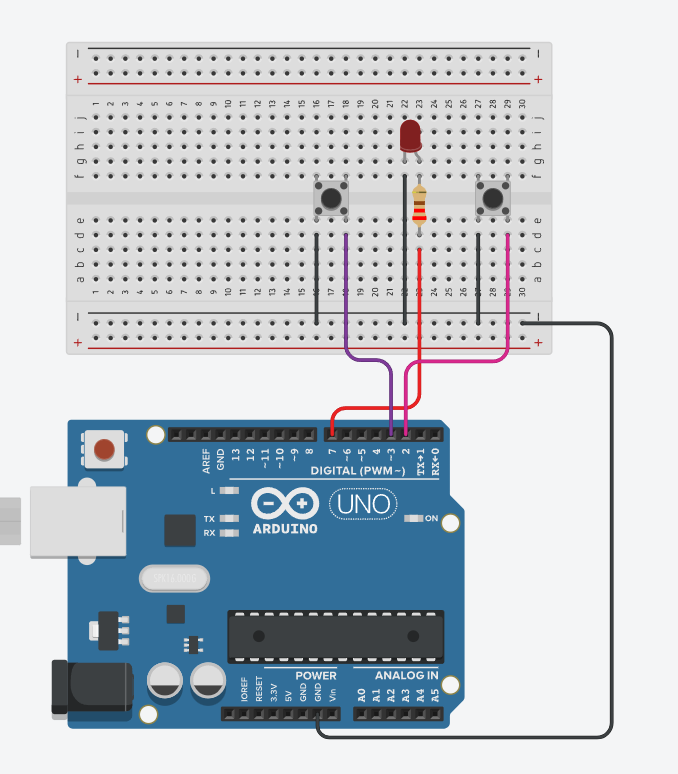
\includegraphics[width=17cm]{z1/1.png}
	\caption{схема сборки}
\end{figure}
\begin{figure}[H]
	\centering
	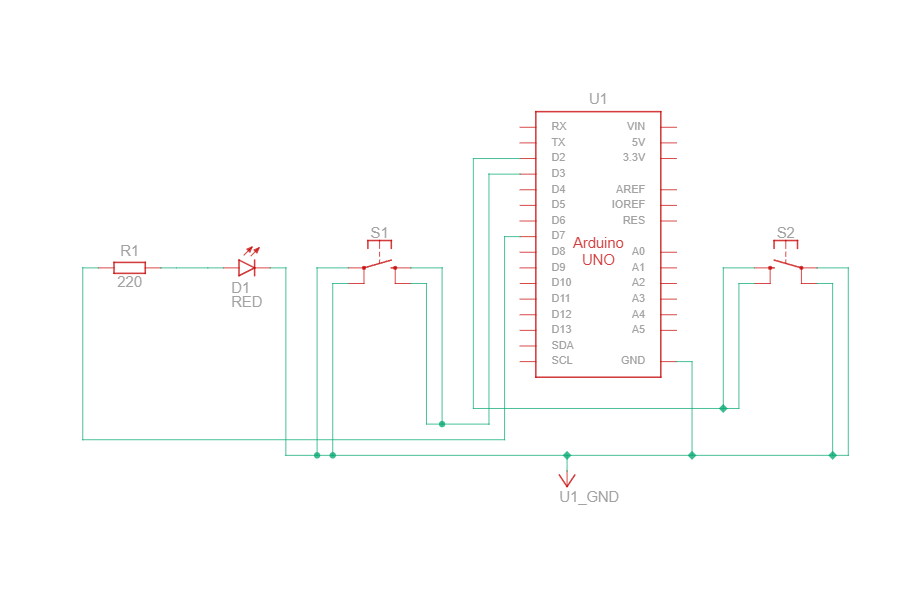
\includegraphics[width=17cm]{z1/2.png}
	\caption{принципиальная схема}
\end{figure}
Код прошивки:
\inputminted{cpp}{z1/main.cpp}
Переменные отвечают за текущее состояние кнопок и предыдущее. При нажатии Левой и Правой или Правой и Левой кнопки последовательно - включается, при нажатии Левой - выключается.
https://www.tinkercad.com/things/6tjt1Z2mn7l-laba-1-zadacha-1
\section{RGB светодиод}
\begin{verbatim}
	Фиксация: да
	Срабатывание: по отпусканию
	Смешивание цветов: нет
	Светодиод с общим: катодом
\end{verbatim}
\begin{figure}[H]
	\centering
	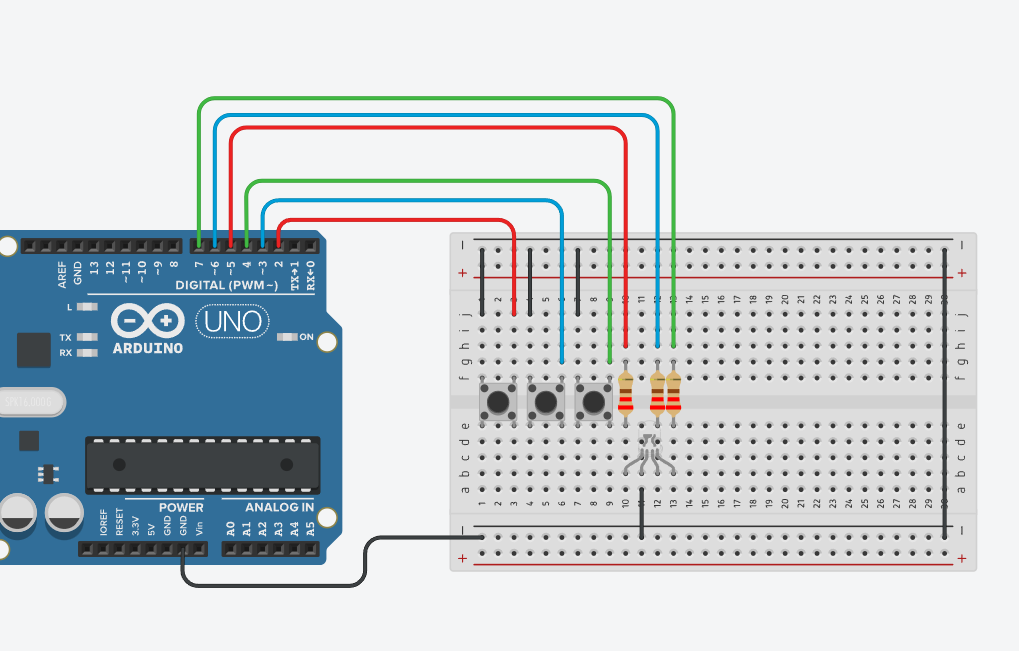
\includegraphics[width=17cm]{z2/1.png}
	\caption{схема сборки}
\end{figure}
\begin{figure}[H]
	\centering
	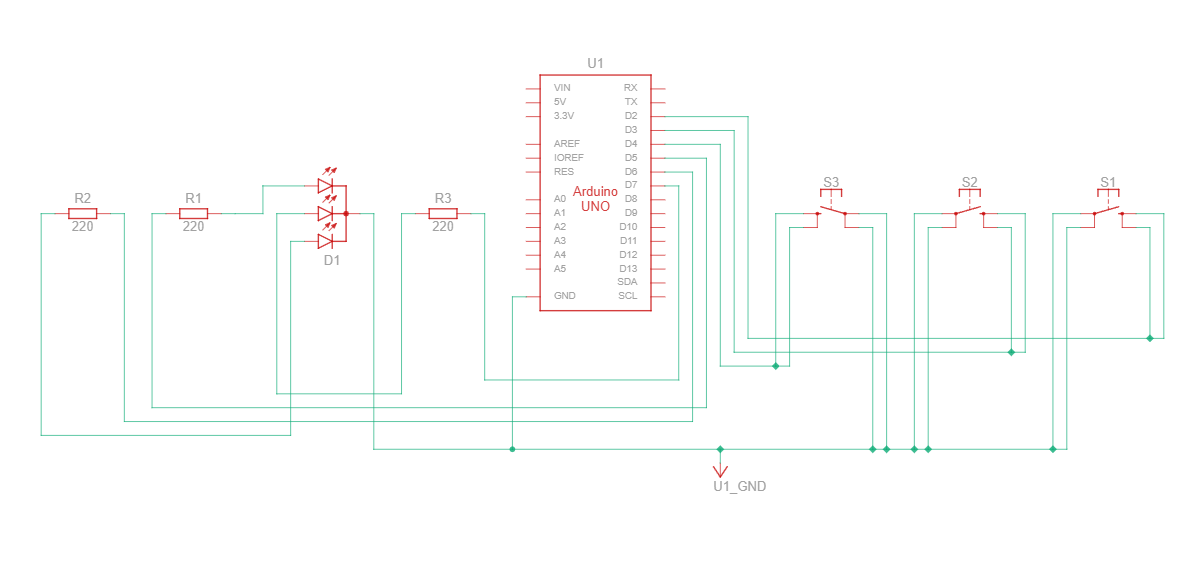
\includegraphics[width=17cm]{z2/2.png}
	\caption{принципиальная схема}
\end{figure}
Код прошивки:
\inputminted{cpp}{z2/main.cpp}
Код управляет RGB-светодиодом с помощью трех кнопок, каждая из которых отвечает за свой цвет, гарантируя, что одновременно горит только один из них (цвета не смешиваются). При отпускании кнопки (с защитой от дребезга контактов в 20 мс) переменная active запоминает индекс этого цвета, а функция update() включает соответствующий светодиод и выключает остальные. Если нажать уже активную кнопку, переменная active сбрасывается в значение 255, и все светодиоды выключаются.
https://www.tinkercad.com/things/8OqotijjY6S-laba-1-zadacha-2
\section{Перетягивание каната}
\begin{verbatim}
	Подключение кнопок: подтягивающий резистор
	Выигрыш: Прерывание по нажатию
	Нажатий для перехода на следующий светодиод: 4
\end{verbatim}
\begin{figure}[H]
	\centering
	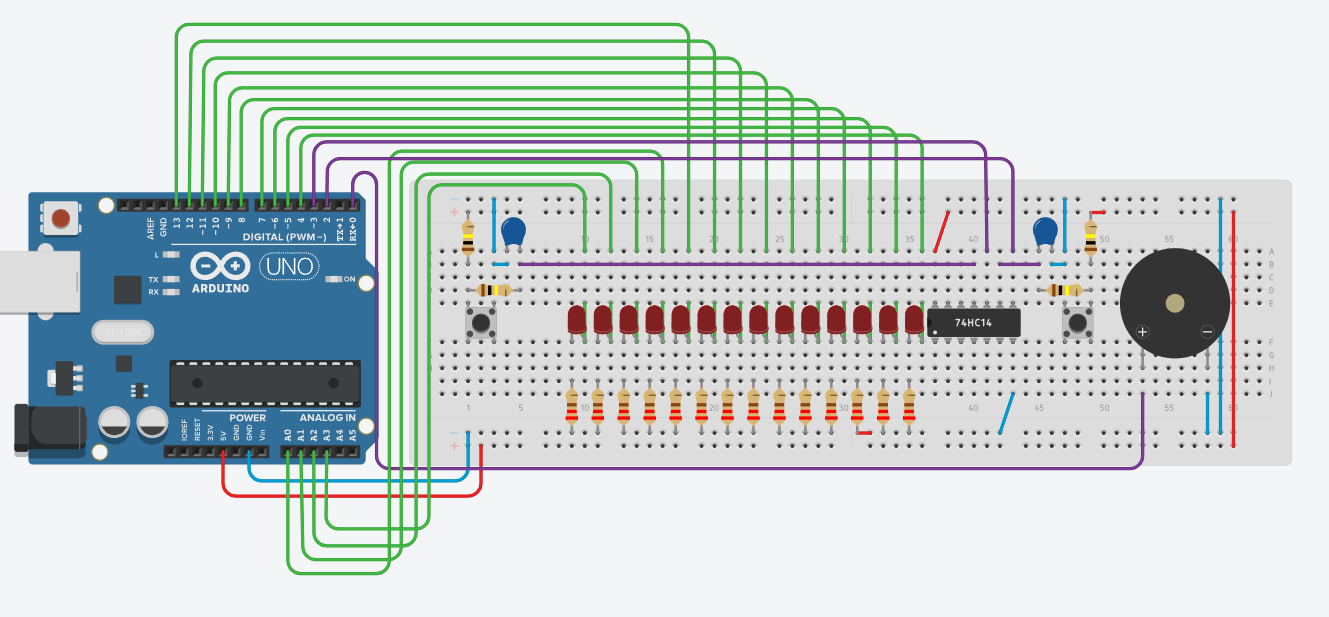
\includegraphics[width=17cm]{z3/1.png}
	\caption{схема сборки}
\end{figure}
\begin{figure}[H]
	\centering
	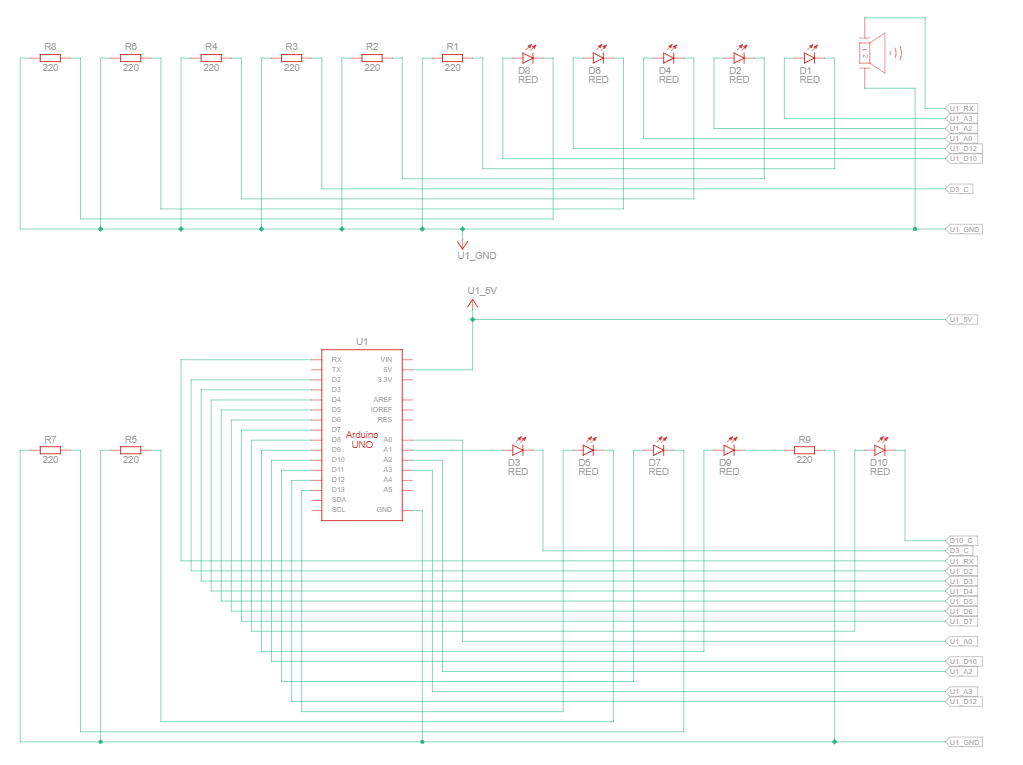
\includegraphics[width=17cm]{z3/2.png}
	\caption{принципиальная схема}
\end{figure}
\begin{figure}[H]
	\centering
	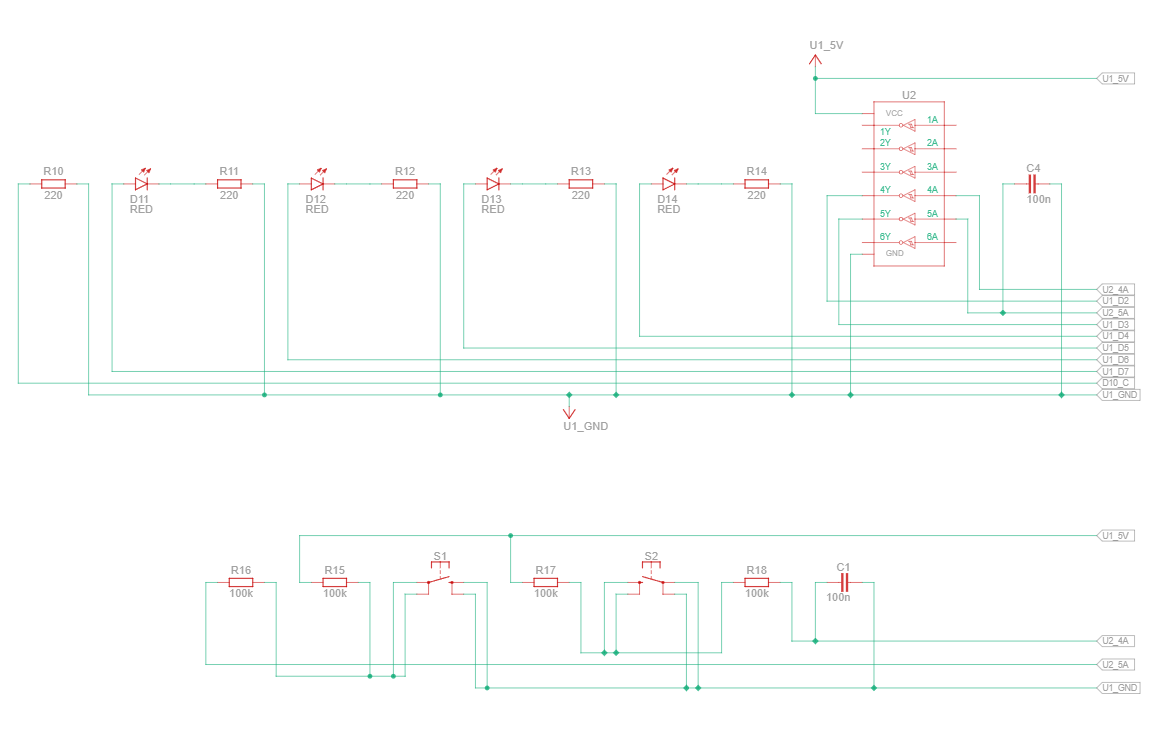
\includegraphics[width=17cm]{z3/3.png}
	\caption{принципиальная схема}
\end{figure}
Код прошивки:
\inputminted{cpp}{z3/main.cpp}
В функциях "pushP1"\ и "pushP2"\ сдвигается счёт в лево или право. В основном цикле программы реализовано отображение счёта на светодиодах (счёт инициализирован с двумя светодиодами по центру, чтобы ни у кого небыло преимущества).
https://www.tinkercad.com/things/0oriWR5BPiA-laba-1-zadacha-3
\section{Логический симулятор}
\begin{verbatim}
	Логическая функция: XOR
	Формула: A, B (2 кнопки)
	Пояснение: Горит, если нажата ТОЛЬКО одна из двух
\end{verbatim}
\begin{figure}[H]
	\centering
	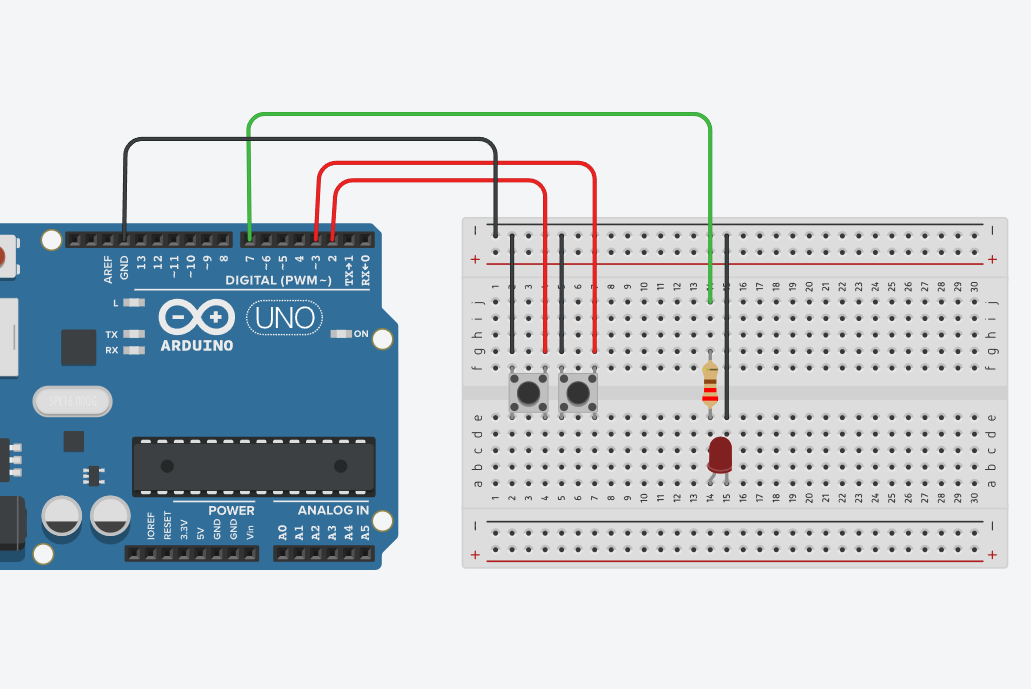
\includegraphics[width=17cm]{z4/1.png}
	\caption{схема сборки}
\end{figure}
\begin{figure}[H]
	\centering
	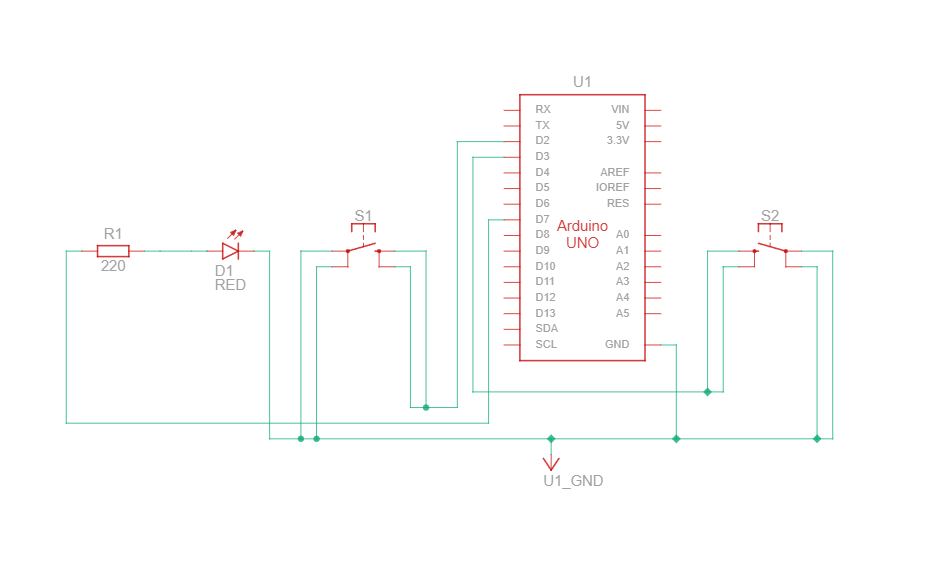
\includegraphics[width=17cm]{z4/2.png}
	\caption{принципиальная схема}
\end{figure}
Код прошивки:
\inputminted{cpp}{z4/main.cpp}
Вводится "a"\ , "b"\  и "c"\ инвертированный сигнал с кнопок, подключенных через встроенный подтягивающий резистор. В запись сигнала на светодиод записано логическое условие через логические операторы.
https://www.tinkercad.com/things/aB05Kq17s2K-laba-1-zadacha-4